\documentclass[11pt]{article}
\usepackage{geometry,marginnote} % Pour passer au format A4
\geometry{hmargin=1cm, vmargin=1cm} % 

% Page et encodage
\usepackage[T1]{fontenc} % Use 8-bit encoding that has 256 glyphs
\usepackage[english,french]{babel} % Français et anglais
\usepackage[utf8]{inputenc} 

\usepackage{lmodern,numprint}
\setlength\parindent{0pt}

% Graphiques
\usepackage{graphicx,float,grffile,units}
\usepackage{tikz,pst-eucl,pst-plot,pstricks,pst-node,pstricks-add,pst-fun} 

% Maths et divers
\usepackage{amsmath,amsfonts,amssymb,amsthm,verbatim}
\usepackage{multicol,enumitem,url,eurosym,gensymb,tabularx}

\DeclareUnicodeCharacter{20AC}{\euro}



% Sections
\usepackage{sectsty} % Allows customizing section commands
\allsectionsfont{\centering \normalfont\scshape}

% Tête et pied de page
\usepackage{fancyhdr} \pagestyle{fancyplain} \fancyhead{} \fancyfoot{}

\renewcommand{\headrulewidth}{0pt} % Remove header underlines
\renewcommand{\footrulewidth}{0pt} % Remove footer underlines

\newcommand{\horrule}[1]{\rule{\linewidth}{#1}} % Create horizontal rule command with 1 argument of height

\newcommand{\Pointilles}[1][3]{%
  \multido{}{#1}{\makebox[\linewidth]{\dotfill}\\[\parskip]
}}

\newtheorem{Definition}{Définition}

\usepackage{siunitx}
\sisetup{
    detect-all,
    output-decimal-marker={,},
    group-minimum-digits = 3,
    group-separator={~},
    number-unit-separator={~},
    inter-unit-product={~}
}

\setlength{\columnseprule}{1pt}

\begin{document}

\horrule{2px}
\section*{Chapitre 4 - Nombres relatifs}
\horrule{2px}

\section*{Où trouve-t-on des nombres négatifs ?}

Les nombres négatifs ne se trouve pas de partout. Ils sont néanmoins assez courants.

\textit{Remarque : négatif vient du latin \textbf{negare} qui signifie nier.}

\begin{multicols}{2}
\begin{enumerate}
  \item[1.] La température.
  \begin{figure}[H]
    \centering
    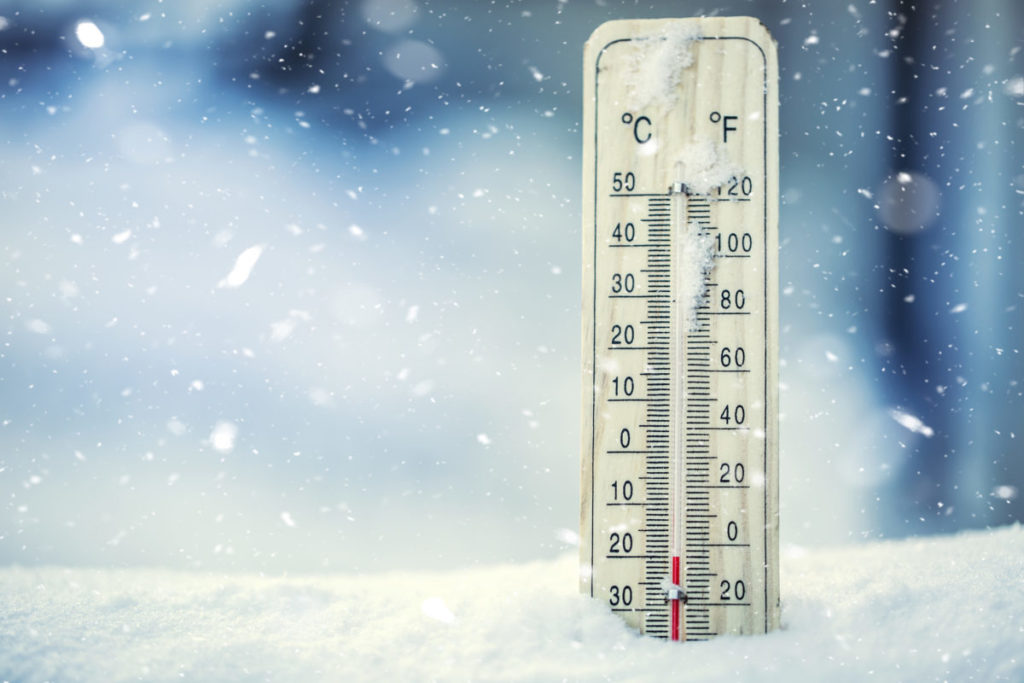
\includegraphics[width=0.8\linewidth]{5x4-relatifs/c-temp.png}
  \end{figure}
  \item[2.] L'altitude sous la mer.
  \begin{figure}[H]
    \centering
    
\includegraphics[width=0.8\linewidth]{5x4-relatifs/c-plongee.png}
  \end{figure}
\end{enumerate}
\end{multicols}


  \begin{multicols}{2}
    \begin{enumerate}
  \item[3.] Les étages d'ascenseurs.
  \begin{figure}[H]
    \centering
    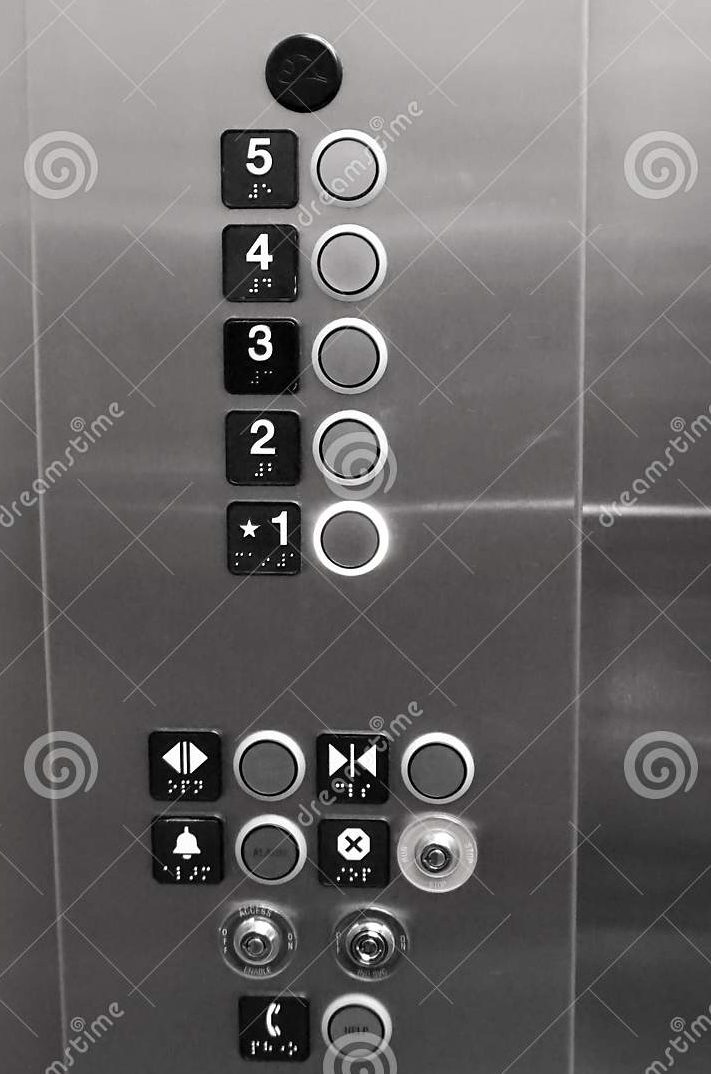
\includegraphics[width=0.8\linewidth]{5x4-relatifs/c-ascenseur.png}
  \end{figure}
  \item[4.] Les dettes d'argents. 
  \begin{figure}[H]
    \centering
    
\includegraphics[width=0.8\linewidth]{5x4-relatifs/c-argent.png}
  \end{figure}
  \item[5.] En électricité. 
  \begin{figure}[H]
    \centering
    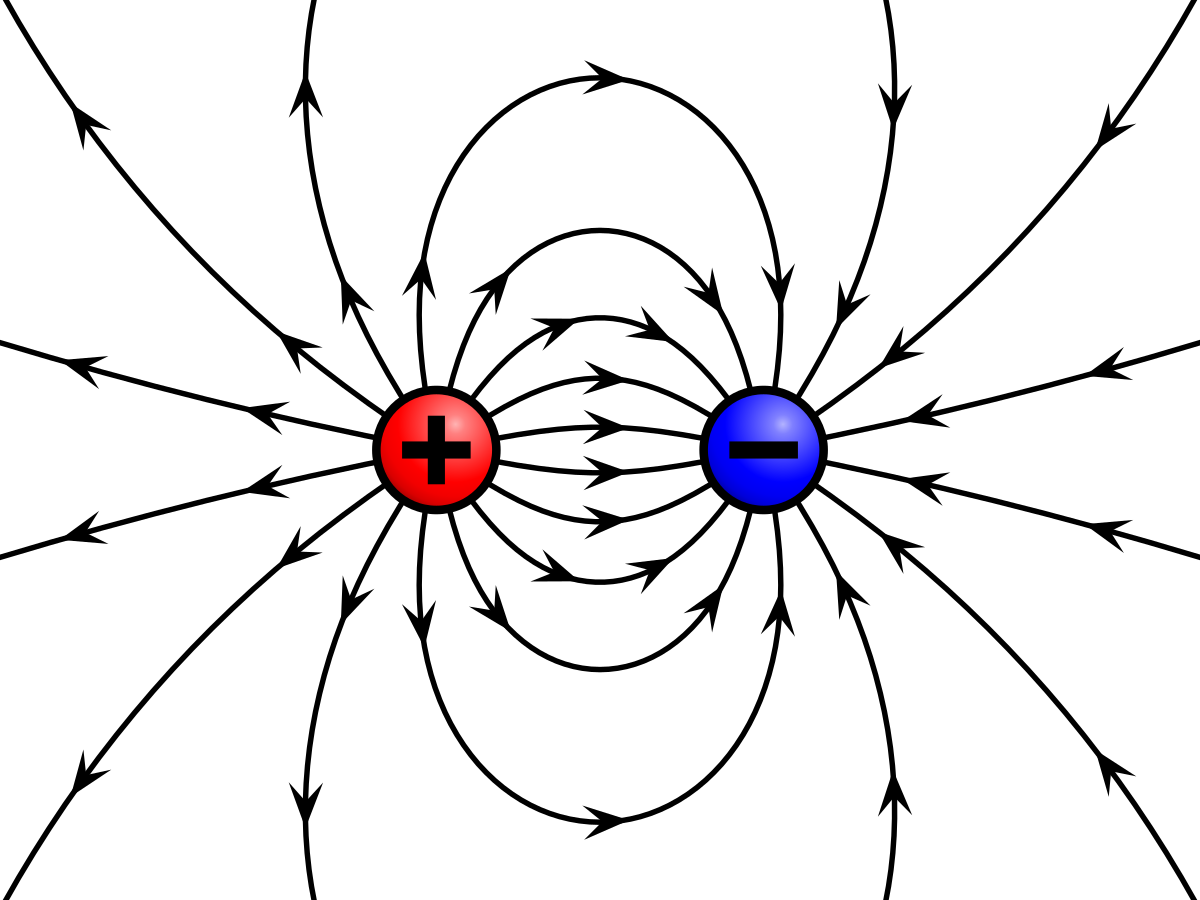
\includegraphics[width=0.8\linewidth]{5x4-relatifs/c-elec.png}
  \end{figure} 
\end{enumerate}
\end{multicols}

\newpage

\section*{1 - Le vocabulaire}


\begin{Definition}{Un nombre négatif}\\
  Un nombre négatif est un nombre plus petit que 0.
\end{Definition}

\begin{Definition}{Les entiers relatifs}\\
  L'ensemble des entiers relatifs est l'ensemble des nombres entiers positifs et négatifs. 
\end{Definition}

\section*{2 - D'abord les points}

\subsection*{1. La droite graduée}

\begin{figure}[H]
  \centering
  \includegraphics[width=0.8\linewidth]{5x4-relatifs/c-axe-1.pdf}
\end{figure}

\begin{Definition}{Abscisse d'un point}\\
  L'abscisse d'un point est la position du point sur la droite. Il suffit de lire la graduation.\\
  On appelle O : \textbf{l'origine} du repère : le 0.
\end{Definition}


\begin{itemize}[label={$\bullet$}]
  \item \textbf{Les nombres à droite de 0 sont positifs.} Plus ils sont à droite, plus ils sont grands. 
  \item \textbf{Les nombres à gauche de 0 sont négatifs.} Plus ils sont à gauche, plus ils sont petits.
\end{itemize}   

\subsection*{2. L'écriture}

On a besoin d'une nouvelle notation pour écrire les nombres négatifs. On utilise le symbole $-$.\\

Ex : $-5$ signifie que le nombre est plus petit que $0$ de $5$.

\begin{Definition}{Distance d'un point à 0}\\
  La distance d'un point à 0 est la longueur qui sépare le point de 0.
\end{Definition}

\subsection*{3. La comparaison}

\begin{itemize}[label={$\bullet$}]
  \item $ -20 < 5$ : un nombre positif est toujours plus grand qu'un nombre négatif.
  \item $ -20 < -8$ : avec les négatifs, plus la distance à zéro est grande, plus le nombre est petit.
  \item $ -8,2 < -8,12$ : cela reste vraie avec les nombres décimaux.
\end{itemize}   


\section*{3 - Enfin les nombres}

\begin{Definition}{Opposé}\\
  Deux nombres sont opposés si leur somme est nulle. 
\end{Definition}

 $-5$ est l'opposé de $5$ : La somme de $-5$ et $5$ est égale à $0$.

\begin{itemize}[label={$\bullet$}]
  \item $-5 + 5 = 0$
  \item $5 + -5 = 0$ 
\end{itemize} 

Ex : $2$ et $-2$ ; $-7$ et $7$ ; $-300$ et $300$ ; ... \\

\textbf{Conclusion : }

\begin{itemize}[label={$\bullet$}]
  \item En ajoutant un nombre négatif le résultat est plus petit. 
  \item Avec ces nouveaux nombres, on va devoir apprendre / compléter / redonner du sens aux opérations : $+$; $-$ ; $\times$ et $\div$. (prochain chapitre)
\end{itemize} 

\end{document}
